\section{Princípio da Indução Finita}

O Princípio da indução finita é um Teorema muito usado. Nosso objetivo não é demonstrá-lo. Queremos usá-lo em situações e problemas mais elementares para possibilitar o entendimento e uso básico dessa poderosa ferramenta.

\begin{theorem}[Princípio da Indução Finita]
\label{theorem:pif}
Considere $n_0$ um inteiro não negativo. Suponhamos que, para cada inteiro $n \geq n_0$, seja dada uma proposição $p \prn n$. Suponha
que se pode verificar as seguintes propriedades:

\begin{enumerate}[(a)]
  \item $p \prn{n_0}$ é verdadeira;
  \item Se $p \prn n$ é verdadeira, então $p \prn {n+1}$ também
  é verdadeira, para todo $n \geq n_0$.
\end{enumerate}

\noindent Então, $p \prn n$ é verdadeira para qualquer $n \geq n_0$.
\end{theorem}

\begin{remark}
No Teorema \ref{theorem:pif}, a afirmação (a) é chamada de \textdef{base da indução}, e a (b), de \textdef{passo indutivo}. O fato de que $p \prn n$ é verdadeira no item (b) é chamado de \textdef{hipótese de indução}.
\end{remark}

\begin{example}
Demonstre que, para qualquer $n \in \N^*$, é válida a igualdade:
%
$$2+ 4+ \dots + 2n = n \prn {n+1}.$$
\end{example}


\begin{solution}
	A fim de provar que a soma dos $n$ primeiros números pares é igual a $n(n+1)$, ou seja, $2+4+\dots + 2n = n(n+1)$ para todo $n \in \nnats$, aplicaremos indução em $n$.
	
	\case{Caso base $[n=1]$}
	Observe que $2 = 1(1+1)$, ou seja, a soma do primeiro número par (somente o 2) é igual a $1(1+1)$. Logo, o caso base é válido.
	
	\case{Passo indutivo}
	Suponha, como Hipótese de Indução (HI), que para algum $n \in \nnats$, vale a equação:
	$$2+4+\dots+2n=n(n+1).$$
	Provemos então que:
	$$2+4+\dots + 2n + 2(n+1) = (n+1)[(n+1)+1].$$
	De fato, segue da (HI) que:
	\begin{align*}
	\underbrace{2+4+\dots+2n}_{\text{HI}} +2(n+1)	&= \underbrace{n(n+1)}_{\text{HI}} + 2(n+1) \\
	&= (n+1)(n+2) \\
	&= (n+1)[(n+1)+1].
	\end{align*}
	Com isso, concluímos que o passo indutivo é satisfeito.
	Portanto, pelo Princípio da Indução Finita, a equação $2+4+\dots + 2n=n(n+1)$ é válida para todo $n \in \nnats$.
	\end{solution}


\begin{example}
Demonstre que, para qualquer $n \in \N^*$, é válida a igualdade:
$$1+3+\dots +\prn {2n-1} = n^2.$$
\end{example}

\begin{solution}
Demonstremos que a igualdade vale aplicando Indução em $n$.

\case{Caso base $[n=1]$}
Como $1=1^2$, o caso base é válido.

\case{Passo indutivo}
Assuma, como Hipótese de Indução (HI), que a igualdade vale para algum $n\in \nnats$, ou seja:
$$1+3+\dots+(2n-1) = n^2.$$
Provemos a validade da equação:
$$1+3+\dots+(2n-1)+[2(n+1)-1] = (n+1)^2.$$
Calculando o lado esquerdo da igualdade, obtemos:
\begin{align*}
\underbrace{1+3+\dots+(2n-1)}_{\text{HI}} + [2(n+1)-1] & = \underbrace{n^2}_{\text{HI}} + 2n + 1 \\
& = (n + 1)^2
\end{align*}
Com isso, provamos que o passo indutivo é válido.
Portanto $p(n)$ vale para todo $n \in \nnats$.
\end{solution}

\begin{example}
Mostre que, para todo número $n \in \nnats$ tal que $n>3$ vale:
$$2^n < n!$$
\end{example}

\begin{solution}
Considere $n \in \nnats$ tal que $n >3$. Provemos que $2^n < n!$ aplicando Indução em $n$.

\case{Caso base $[n=4]$} Temos $2^4 = 16$ e $4! = 24$. Como $16 < 24$, o caso base é satisfeito.

\case{Passo Indutivo}
Suponha, como Hipótese de Indução, que vale $2^n < n!$ para algum $n \in \nnats$ tal que $n > 3$.

Provemos que vale $2^{n+1} < (n+1)!$.
Inicialmente, observe que $2 < n + 1$, visto que $2 < 3 < n < n + 1$. Também temos que $2$ e $2^n$ são positivos. Sendo assim, podemos concluir que:
\begin{align*}
2^n < n! \text{ e } 2 < n+1 & \implies 2^n \cdot 2 < n!(n+1) \\
& \implies 2^{n+1} < (n+1)!.
\end{align*}
Assim provando que vale o passo indutivo.
Portanto, $2^n < n!$ para qualquer $n \in \nnats$ tal que $n>3$.
\end{solution}

\begin{example}
Prove  que, para todo $n \in \nnats$,
%
\begin{equation*}
\underbrace{\sqrt{2+\sqrt{2+\sqrt{2+ \dots + \sqrt 2}}}}_{n  \text{ radicais}} < 2.
\end{equation*}
\end{example}

\begin{solution}
Aplicaremos o Princípio da Indução Finita em $n \in \nnats$.
%
\begin{itemize}
	\item \textit{Caso base} ($n=1$):

	$\sqrt 2 < 2$ é válido.

	\item \textit{Passo indutivo}:

	Suponha a validade da inequação para algum $k \in \nnats$, ou seja, 
	%
	\begin{equation*}
	\underbrace{\sqrt{2+\sqrt{2+\sqrt{2+ \dots + \sqrt 2}}}}_{k  \text{ radicais}} < 2.
	\end{equation*}
	%
	Da hipótese de indução, segue que:
	%
	\begin{align*}
	2+\underbrace{\sqrt{2+\sqrt{2+\sqrt{2+ \dots + \sqrt 2}}}}_{k  \text{ radicais}} < 2+2 & \implies \underbrace{\sqrt{2+\sqrt{2+\sqrt{2+ \dots + \sqrt 2}}}}_{k+1  \text{ radicais}} < \sqrt 4 = 2.
	\end{align*}
\end{itemize}
%
Logo, a inequação é válida para $n = k+1$; e, assim, concluímos a validade da inequação para todo $n \in \nnats$.
\end{solution}

\begin{example}
Seja $n \in \N$ tal que $n\ge 3$. Mostre  que podemos cobrir os $n^2$ pontos no reticulado a seguir traçando $2n-2$ segmentos de reta sem tirar o lápis do papel.
%
\begin{equation*}
\underbrace{\begin{array}{ccccc}
                \bullet & \bullet & \bullet & \bullet & \bullet \\
                \bullet & \bullet & \bullet & \bullet & \bullet \\
                \bullet & \bullet & \bullet & \bullet & \bullet \\
                \bullet & \bullet & \bullet & \bullet & \bullet \\
                \bullet & \bullet & \bullet & \bullet & \bullet
              \end{array}
}_{n \times n \text{ pontos}}
\end{equation*}
\begin{solution}
	Aplicaremos indução finita em $n \ge 3$, valor que determina a quantidade de pontos do reticulado e de segmentos de reta que podem ser utilizados.
	\begin{itemize}
		\item \textit{Caso base}[$n = 3$]: Uma solução usando $2\cdot 3 -2 = 4$ segmentos de reta sem tirar o lápis do papel pode ser vista na figura abaixo.

		\begin{center}
		\tikzset{every picture/.style={line width=0.75pt}} %set default line width to 0.75pt        

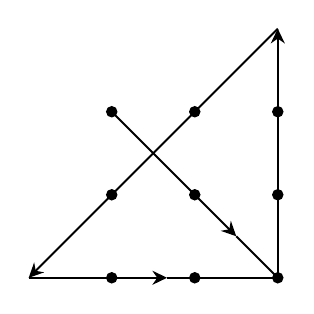
\begin{tikzpicture}[x=0.5pt,y=0.5pt,yscale=-1,xscale=1]
%uncomment if require: \path (0,235); %set diagram left start at 0, and has height of 235

%Straight Lines [id:da9313950171592851] 
\draw [color={rgb, 255:red, 0; green, 0; blue, 0 }  ,draw opacity=1 ][line width=0.75]    (270,90) -- (358.59,178.59) ;
\draw [shift={(360,180)}, rotate = 225] [fill={rgb, 255:red, 0; green, 0; blue, 0 }  ,fill opacity=1 ][line width=0.75]  [draw opacity=0] (10.72,-5.15) -- (0,0) -- (10.72,5.15) -- (7.12,0) -- cycle    ;

%Straight Lines [id:da11085152369049278] 
\draw [color={rgb, 255:red, 0; green, 0; blue, 0 }  ,draw opacity=1 ][line width=0.75]    (390,210) -- (390,32) ;
\draw [shift={(390,30)}, rotate = 450] [fill={rgb, 255:red, 0; green, 0; blue, 0 }  ,fill opacity=1 ][line width=0.75]  [draw opacity=0] (10.72,-5.15) -- (0,0) -- (10.72,5.15) -- (7.12,0) -- cycle    ;

%Straight Lines [id:da18764486170935302] 
\draw [color={rgb, 255:red, 0; green, 0; blue, 0 }  ,draw opacity=1 ][line width=0.75]    (390,30) -- (211.41,208.59) ;
\draw [shift={(210,210)}, rotate = 315] [fill={rgb, 255:red, 0; green, 0; blue, 0 }  ,fill opacity=1 ][line width=0.75]  [draw opacity=0] (10.72,-5.15) -- (0,0) -- (10.72,5.15) -- (7.12,0) -- cycle    ;

%Straight Lines [id:da9197089608689861] 
\draw [color={rgb, 255:red, 0; green, 0; blue, 0 }  ,draw opacity=1 ][line width=0.75]    (210,210) -- (308,210) ;
\draw [shift={(310,210)}, rotate = 180] [fill={rgb, 255:red, 0; green, 0; blue, 0 }  ,fill opacity=1 ][line width=0.75]  [draw opacity=0] (10.72,-5.15) -- (0,0) -- (10.72,5.15) -- (7.12,0) -- cycle    ;

%Straight Lines [id:da7972297216274716] 
\draw [color={rgb, 255:red, 0; green, 0; blue, 0 }  ,draw opacity=1 ][line width=0.75]    (330,150) ;

\draw [shift={(330,150)}, rotate = 0] [color={rgb, 255:red, 0; green, 0; blue, 0 }  ,draw opacity=1 ][fill={rgb, 255:red, 0; green, 0; blue, 0 }  ,fill opacity=1 ][line width=0.75]      (0, 0) circle [x radius= 3.35, y radius= 3.35]   ;
%Straight Lines [id:da2575684081280536] 
\draw [color={rgb, 255:red, 0; green, 0; blue, 0 }  ,draw opacity=1 ][line width=0.75]    (360,180) -- (390,210) ;


%Straight Lines [id:da5664811159800692] 
\draw [color={rgb, 255:red, 0; green, 0; blue, 0 }  ,draw opacity=1 ][line width=0.75]    (390,150) ;

\draw [shift={(390,150)}, rotate = 0] [color={rgb, 255:red, 0; green, 0; blue, 0 }  ,draw opacity=1 ][fill={rgb, 255:red, 0; green, 0; blue, 0 }  ,fill opacity=1 ][line width=0.75]      (0, 0) circle [x radius= 3.35, y radius= 3.35]   ;
%Straight Lines [id:da8353908393907012] 
\draw [color={rgb, 255:red, 0; green, 0; blue, 0 }  ,draw opacity=1 ][line width=0.75]    (270,150) ;

\draw [shift={(270,150)}, rotate = 0] [color={rgb, 255:red, 0; green, 0; blue, 0 }  ,draw opacity=1 ][fill={rgb, 255:red, 0; green, 0; blue, 0 }  ,fill opacity=1 ][line width=0.75]      (0, 0) circle [x radius= 3.35, y radius= 3.35]   ;
%Straight Lines [id:da5265109832105077] 
\draw [color={rgb, 255:red, 0; green, 0; blue, 0 }  ,draw opacity=1 ][line width=0.75]    (330,90) ;

\draw [shift={(330,90)}, rotate = 0] [color={rgb, 255:red, 0; green, 0; blue, 0 }  ,draw opacity=1 ][fill={rgb, 255:red, 0; green, 0; blue, 0 }  ,fill opacity=1 ][line width=0.75]      (0, 0) circle [x radius= 3.35, y radius= 3.35]   ;
%Straight Lines [id:da5880496172127448] 
\draw [color={rgb, 255:red, 0; green, 0; blue, 0 }  ,draw opacity=1 ][line width=0.75]    (330,210) ;

\draw [shift={(330,210)}, rotate = 0] [color={rgb, 255:red, 0; green, 0; blue, 0 }  ,draw opacity=1 ][fill={rgb, 255:red, 0; green, 0; blue, 0 }  ,fill opacity=1 ][line width=0.75]      (0, 0) circle [x radius= 3.35, y radius= 3.35]   ;
%Straight Lines [id:da6858460611860261] 
\draw [color={rgb, 255:red, 0; green, 0; blue, 0 }  ,draw opacity=1 ][line width=0.75]    (270,210) ;

\draw [shift={(270,210)}, rotate = 0] [color={rgb, 255:red, 0; green, 0; blue, 0 }  ,draw opacity=1 ][fill={rgb, 255:red, 0; green, 0; blue, 0 }  ,fill opacity=1 ][line width=0.75]      (0, 0) circle [x radius= 3.35, y radius= 3.35]   ;
%Straight Lines [id:da2843750828207233] 
\draw [color={rgb, 255:red, 0; green, 0; blue, 0 }  ,draw opacity=1 ][line width=0.75]    (390,90) ;

\draw [shift={(390,90)}, rotate = 0] [color={rgb, 255:red, 0; green, 0; blue, 0 }  ,draw opacity=1 ][fill={rgb, 255:red, 0; green, 0; blue, 0 }  ,fill opacity=1 ][line width=0.75]      (0, 0) circle [x radius= 3.35, y radius= 3.35]   ;
%Straight Lines [id:da7193275765590325] 
\draw [color={rgb, 255:red, 0; green, 0; blue, 0 }  ,draw opacity=1 ][line width=0.75]    (310,210) -- (390,210) ;


%Straight Lines [id:da9588395335059182] 
\draw [color={rgb, 255:red, 0; green, 0; blue, 0 }  ,draw opacity=1 ][line width=0.75]    (270,90) ;

\draw [shift={(270,90)}, rotate = 0] [color={rgb, 255:red, 0; green, 0; blue, 0 }  ,draw opacity=1 ][fill={rgb, 255:red, 0; green, 0; blue, 0 }  ,fill opacity=1 ][line width=0.75]      (0, 0) circle [x radius= 3.35, y radius= 3.35]   ;
%Straight Lines [id:da7877176027665432] 
\draw [color={rgb, 255:red, 0; green, 0; blue, 0 }  ,draw opacity=1 ][line width=0.75]    (390,210) ;

\draw [shift={(390,210)}, rotate = 0] [color={rgb, 255:red, 0; green, 0; blue, 0 }  ,draw opacity=1 ][fill={rgb, 255:red, 0; green, 0; blue, 0 }  ,fill opacity=1 ][line width=0.75]      (0, 0) circle [x radius= 3.35, y radius= 3.35]   ;

\end{tikzpicture}

		\end{center}
		
		\item \textit{Passo indutivo}: Para a demonstração do passo indutivo, fugiremos um pouco do modelo que estamos apresentando até então e apresentaremos como a solução para o caso $n = 3$ nos traz a solução para o caso $n = 4$ e desse, para o caso $n=5$. Isto a fim de mostrar que através da repetição do método, a solução para algum $n \ge 3$ implica na solução para $n+1$.
		
		\begin{center}
		\tikzset{every picture/.style={line width=0.75pt}} %set default line width to 0.75pt        

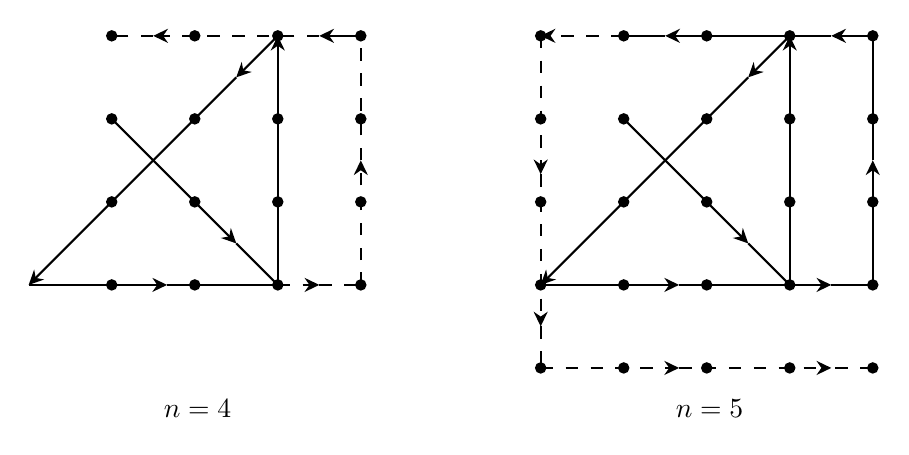
\begin{tikzpicture}[x=0.5pt,y=0.5pt,yscale=-1,xscale=1]
%uncomment if require: \path (0,308.4499969482422); %set diagram left start at 0, and has height of 308.4499969482422

%Straight Lines [id:da9313950171592851] 
\draw [color={rgb, 255:red, 0; green, 0; blue, 0 }  ,draw opacity=1 ][line width=0.75]    (80,90) -- (168.59,178.59) ;
\draw [shift={(170,180)}, rotate = 225] [fill={rgb, 255:red, 0; green, 0; blue, 0 }  ,fill opacity=1 ][line width=0.75]  [draw opacity=0] (10.72,-5.15) -- (0,0) -- (10.72,5.15) -- (7.12,0) -- cycle    ;

%Straight Lines [id:da11085152369049278] 
\draw [color={rgb, 255:red, 0; green, 0; blue, 0 }  ,draw opacity=1 ][line width=0.75]    (200,210) -- (200,32) ;
\draw [shift={(200,30)}, rotate = 450] [fill={rgb, 255:red, 0; green, 0; blue, 0 }  ,fill opacity=1 ][line width=0.75]  [draw opacity=0] (10.72,-5.15) -- (0,0) -- (10.72,5.15) -- (7.12,0) -- cycle    ;

%Straight Lines [id:da18764486170935302] 
\draw [color={rgb, 255:red, 0; green, 0; blue, 0 }  ,draw opacity=1 ][line width=0.75]    (200,30) -- (171.41,58.59) ;
\draw [shift={(170,60)}, rotate = 315] [fill={rgb, 255:red, 0; green, 0; blue, 0 }  ,fill opacity=1 ][line width=0.75]  [draw opacity=0] (10.72,-5.15) -- (0,0) -- (10.72,5.15) -- (7.12,0) -- cycle    ;

%Straight Lines [id:da9197089608689861] 
\draw [color={rgb, 255:red, 0; green, 0; blue, 0 }  ,draw opacity=1 ][line width=0.75]    (20,210) -- (118,210) ;
\draw [shift={(120,210)}, rotate = 180] [fill={rgb, 255:red, 0; green, 0; blue, 0 }  ,fill opacity=1 ][line width=0.75]  [draw opacity=0] (10.72,-5.15) -- (0,0) -- (10.72,5.15) -- (7.12,0) -- cycle    ;

%Straight Lines [id:da7972297216274716] 
\draw [color={rgb, 255:red, 0; green, 0; blue, 0 }  ,draw opacity=1 ][line width=0.75]    (140,150) ;

\draw [shift={(140,150)}, rotate = 0] [color={rgb, 255:red, 0; green, 0; blue, 0 }  ,draw opacity=1 ][fill={rgb, 255:red, 0; green, 0; blue, 0 }  ,fill opacity=1 ][line width=0.75]      (0, 0) circle [x radius= 3.35, y radius= 3.35]   ;
%Straight Lines [id:da2575684081280536] 
\draw [color={rgb, 255:red, 0; green, 0; blue, 0 }  ,draw opacity=1 ][line width=0.75]    (170,180) -- (200,210) ;


%Straight Lines [id:da5664811159800692] 
\draw [color={rgb, 255:red, 0; green, 0; blue, 0 }  ,draw opacity=1 ][line width=0.75]    (200,150) ;

\draw [shift={(200,150)}, rotate = 0] [color={rgb, 255:red, 0; green, 0; blue, 0 }  ,draw opacity=1 ][fill={rgb, 255:red, 0; green, 0; blue, 0 }  ,fill opacity=1 ][line width=0.75]      (0, 0) circle [x radius= 3.35, y radius= 3.35]   ;
%Straight Lines [id:da8353908393907012] 
\draw [color={rgb, 255:red, 0; green, 0; blue, 0 }  ,draw opacity=1 ][line width=0.75]    (80,150) ;

\draw [shift={(80,150)}, rotate = 0] [color={rgb, 255:red, 0; green, 0; blue, 0 }  ,draw opacity=1 ][fill={rgb, 255:red, 0; green, 0; blue, 0 }  ,fill opacity=1 ][line width=0.75]      (0, 0) circle [x radius= 3.35, y radius= 3.35]   ;
%Straight Lines [id:da5265109832105077] 
\draw [color={rgb, 255:red, 0; green, 0; blue, 0 }  ,draw opacity=1 ][line width=0.75]    (140,90) ;

\draw [shift={(140,90)}, rotate = 0] [color={rgb, 255:red, 0; green, 0; blue, 0 }  ,draw opacity=1 ][fill={rgb, 255:red, 0; green, 0; blue, 0 }  ,fill opacity=1 ][line width=0.75]      (0, 0) circle [x radius= 3.35, y radius= 3.35]   ;
%Straight Lines [id:da5880496172127448] 
\draw [color={rgb, 255:red, 0; green, 0; blue, 0 }  ,draw opacity=1 ][line width=0.75]    (140,210) ;

\draw [shift={(140,210)}, rotate = 0] [color={rgb, 255:red, 0; green, 0; blue, 0 }  ,draw opacity=1 ][fill={rgb, 255:red, 0; green, 0; blue, 0 }  ,fill opacity=1 ][line width=0.75]      (0, 0) circle [x radius= 3.35, y radius= 3.35]   ;
%Straight Lines [id:da6858460611860261] 
\draw [color={rgb, 255:red, 0; green, 0; blue, 0 }  ,draw opacity=1 ][line width=0.75]    (80,210) ;

\draw [shift={(80,210)}, rotate = 0] [color={rgb, 255:red, 0; green, 0; blue, 0 }  ,draw opacity=1 ][fill={rgb, 255:red, 0; green, 0; blue, 0 }  ,fill opacity=1 ][line width=0.75]      (0, 0) circle [x radius= 3.35, y radius= 3.35]   ;
%Straight Lines [id:da2843750828207233] 
\draw [color={rgb, 255:red, 0; green, 0; blue, 0 }  ,draw opacity=1 ][line width=0.75]    (200,90) ;

\draw [shift={(200,90)}, rotate = 0] [color={rgb, 255:red, 0; green, 0; blue, 0 }  ,draw opacity=1 ][fill={rgb, 255:red, 0; green, 0; blue, 0 }  ,fill opacity=1 ][line width=0.75]      (0, 0) circle [x radius= 3.35, y radius= 3.35]   ;
%Straight Lines [id:da7193275765590325] 
\draw [color={rgb, 255:red, 0; green, 0; blue, 0 }  ,draw opacity=1 ][line width=0.75]    (120,210) -- (200,210) ;


%Straight Lines [id:da06694861949764497] 
\draw [color={rgb, 255:red, 0; green, 0; blue, 0 }  ,draw opacity=1 ][line width=0.75]  [dash pattern={on 4.5pt off 4.5pt}]  (200,210) -- (228,210) ;
\draw [shift={(230,210)}, rotate = 180] [fill={rgb, 255:red, 0; green, 0; blue, 0 }  ,fill opacity=1 ][line width=0.75]  [draw opacity=0] (10.72,-5.15) -- (0,0) -- (10.72,5.15) -- (7.12,0) -- cycle    ;

%Straight Lines [id:da8639044841447044] 
\draw [color={rgb, 255:red, 0; green, 0; blue, 0 }  ,draw opacity=1 ][line width=0.75]    (260,210) ;

\draw [shift={(260,210)}, rotate = 0] [color={rgb, 255:red, 0; green, 0; blue, 0 }  ,draw opacity=1 ][fill={rgb, 255:red, 0; green, 0; blue, 0 }  ,fill opacity=1 ][line width=0.75]      (0, 0) circle [x radius= 3.35, y radius= 3.35]   ;
%Straight Lines [id:da1632548320523186] 
\draw [color={rgb, 255:red, 0; green, 0; blue, 0 }  ,draw opacity=1 ][line width=0.75]    (260,150) ;

\draw [shift={(260,150)}, rotate = 0] [color={rgb, 255:red, 0; green, 0; blue, 0 }  ,draw opacity=1 ][fill={rgb, 255:red, 0; green, 0; blue, 0 }  ,fill opacity=1 ][line width=0.75]      (0, 0) circle [x radius= 3.35, y radius= 3.35]   ;
%Straight Lines [id:da4095630613489206] 
\draw [color={rgb, 255:red, 0; green, 0; blue, 0 }  ,draw opacity=1 ][line width=0.75]    (260,90) ;

\draw [shift={(260,90)}, rotate = 0] [color={rgb, 255:red, 0; green, 0; blue, 0 }  ,draw opacity=1 ][fill={rgb, 255:red, 0; green, 0; blue, 0 }  ,fill opacity=1 ][line width=0.75]      (0, 0) circle [x radius= 3.35, y radius= 3.35]   ;
%Straight Lines [id:da399089171922975] 
\draw [color={rgb, 255:red, 0; green, 0; blue, 0 }  ,draw opacity=1 ][line width=0.75]    (260,30) ;

\draw [shift={(260,30)}, rotate = 0] [color={rgb, 255:red, 0; green, 0; blue, 0 }  ,draw opacity=1 ][fill={rgb, 255:red, 0; green, 0; blue, 0 }  ,fill opacity=1 ][line width=0.75]      (0, 0) circle [x radius= 3.35, y radius= 3.35]   ;
%Straight Lines [id:da21960861912105245] 
\draw [color={rgb, 255:red, 0; green, 0; blue, 0 }  ,draw opacity=1 ][line width=0.75]    (140,30) ;

\draw [shift={(140,30)}, rotate = 0] [color={rgb, 255:red, 0; green, 0; blue, 0 }  ,draw opacity=1 ][fill={rgb, 255:red, 0; green, 0; blue, 0 }  ,fill opacity=1 ][line width=0.75]      (0, 0) circle [x radius= 3.35, y radius= 3.35]   ;
%Straight Lines [id:da5714938611090269] 
\draw [color={rgb, 255:red, 0; green, 0; blue, 0 }  ,draw opacity=1 ][line width=0.75]    (80,30) ;

\draw [shift={(80,30)}, rotate = 0] [color={rgb, 255:red, 0; green, 0; blue, 0 }  ,draw opacity=1 ][fill={rgb, 255:red, 0; green, 0; blue, 0 }  ,fill opacity=1 ][line width=0.75]      (0, 0) circle [x radius= 3.35, y radius= 3.35]   ;
%Straight Lines [id:da39210283295430426] 
\draw [color={rgb, 255:red, 0; green, 0; blue, 0 }  ,draw opacity=1 ][line width=0.75]  [dash pattern={on 4.5pt off 4.5pt}]  (260,210) -- (260,122) ;
\draw [shift={(260,120)}, rotate = 450] [fill={rgb, 255:red, 0; green, 0; blue, 0 }  ,fill opacity=1 ][line width=0.75]  [draw opacity=0] (10.72,-5.15) -- (0,0) -- (10.72,5.15) -- (7.12,0) -- cycle    ;

%Straight Lines [id:da561716359399634] 
\draw [color={rgb, 255:red, 0; green, 0; blue, 0 }  ,draw opacity=1 ][line width=0.75]  [dash pattern={on 4.5pt off 4.5pt}]  (260,120) -- (260,30) ;


%Straight Lines [id:da7883677598901787] 
\draw [color={rgb, 255:red, 0; green, 0; blue, 0 }  ,draw opacity=1 ][line width=0.75]    (260,30) -- (232,30) ;
\draw [shift={(230,30)}, rotate = 360] [fill={rgb, 255:red, 0; green, 0; blue, 0 }  ,fill opacity=1 ][line width=0.75]  [draw opacity=0] (10.72,-5.15) -- (0,0) -- (10.72,5.15) -- (7.12,0) -- cycle    ;

%Straight Lines [id:da28155600134112624] 
\draw [color={rgb, 255:red, 0; green, 0; blue, 0 }  ,draw opacity=1 ][line width=0.75]  [dash pattern={on 4.5pt off 4.5pt}]  (230,210) -- (260,210) ;


%Straight Lines [id:da4195555165806524] 
\draw [color={rgb, 255:red, 0; green, 0; blue, 0 }  ,draw opacity=1 ][line width=0.75]  [dash pattern={on 4.5pt off 4.5pt}]  (230,30) -- (112,30) ;
\draw [shift={(110,30)}, rotate = 360] [fill={rgb, 255:red, 0; green, 0; blue, 0 }  ,fill opacity=1 ][line width=0.75]  [draw opacity=0] (10.72,-5.15) -- (0,0) -- (10.72,5.15) -- (7.12,0) -- cycle    ;

%Straight Lines [id:da9588395335059182] 
\draw [color={rgb, 255:red, 0; green, 0; blue, 0 }  ,draw opacity=1 ][line width=0.75]    (80,90) ;

\draw [shift={(80,90)}, rotate = 0] [color={rgb, 255:red, 0; green, 0; blue, 0 }  ,draw opacity=1 ][fill={rgb, 255:red, 0; green, 0; blue, 0 }  ,fill opacity=1 ][line width=0.75]      (0, 0) circle [x radius= 3.35, y radius= 3.35]   ;
%Straight Lines [id:da1656649902910805] 
\draw [color={rgb, 255:red, 0; green, 0; blue, 0 }  ,draw opacity=1 ][line width=0.75]    (200,30) ;

\draw [shift={(200,30)}, rotate = 0] [color={rgb, 255:red, 0; green, 0; blue, 0 }  ,draw opacity=1 ][fill={rgb, 255:red, 0; green, 0; blue, 0 }  ,fill opacity=1 ][line width=0.75]      (0, 0) circle [x radius= 3.35, y radius= 3.35]   ;
%Straight Lines [id:da7877176027665432] 
\draw [color={rgb, 255:red, 0; green, 0; blue, 0 }  ,draw opacity=1 ][line width=0.75]    (200,210) ;

\draw [shift={(200,210)}, rotate = 0] [color={rgb, 255:red, 0; green, 0; blue, 0 }  ,draw opacity=1 ][fill={rgb, 255:red, 0; green, 0; blue, 0 }  ,fill opacity=1 ][line width=0.75]      (0, 0) circle [x radius= 3.35, y radius= 3.35]   ;
%Straight Lines [id:da7286121148106096] 
\draw [color={rgb, 255:red, 0; green, 0; blue, 0 }  ,draw opacity=1 ][line width=0.75]    (170,60) -- (21.41,208.59) ;
\draw [shift={(20,210)}, rotate = 315] [fill={rgb, 255:red, 0; green, 0; blue, 0 }  ,fill opacity=1 ][line width=0.75]  [draw opacity=0] (10.72,-5.15) -- (0,0) -- (10.72,5.15) -- (7.12,0) -- cycle    ;

%Straight Lines [id:da13741994406237856] 
\draw [color={rgb, 255:red, 0; green, 0; blue, 0 }  ,draw opacity=1 ][line width=0.75]  [dash pattern={on 4.5pt off 4.5pt}]  (110,30) -- (80,30) ;


%Straight Lines [id:da8267213887286297] 
\draw [color={rgb, 255:red, 0; green, 0; blue, 0 }  ,draw opacity=1 ][line width=0.75]    (390,270) ;

\draw [shift={(390,270)}, rotate = 0] [color={rgb, 255:red, 0; green, 0; blue, 0 }  ,draw opacity=1 ][fill={rgb, 255:red, 0; green, 0; blue, 0 }  ,fill opacity=1 ][line width=0.75]      (0, 0) circle [x radius= 3.35, y radius= 3.35]   ;
%Straight Lines [id:da2726947324927841] 
\draw [color={rgb, 255:red, 0; green, 0; blue, 0 }  ,draw opacity=1 ][line width=0.75]    (390,210) ;

\draw [shift={(390,210)}, rotate = 0] [color={rgb, 255:red, 0; green, 0; blue, 0 }  ,draw opacity=1 ][fill={rgb, 255:red, 0; green, 0; blue, 0 }  ,fill opacity=1 ][line width=0.75]      (0, 0) circle [x radius= 3.35, y radius= 3.35]   ;
%Straight Lines [id:da3412026924167738] 
\draw [color={rgb, 255:red, 0; green, 0; blue, 0 }  ,draw opacity=1 ][line width=0.75]    (390,150) ;

\draw [shift={(390,150)}, rotate = 0] [color={rgb, 255:red, 0; green, 0; blue, 0 }  ,draw opacity=1 ][fill={rgb, 255:red, 0; green, 0; blue, 0 }  ,fill opacity=1 ][line width=0.75]      (0, 0) circle [x radius= 3.35, y radius= 3.35]   ;
%Straight Lines [id:da2869813859441034] 
\draw [color={rgb, 255:red, 0; green, 0; blue, 0 }  ,draw opacity=1 ][line width=0.75]    (390,90) ;

\draw [shift={(390,90)}, rotate = 0] [color={rgb, 255:red, 0; green, 0; blue, 0 }  ,draw opacity=1 ][fill={rgb, 255:red, 0; green, 0; blue, 0 }  ,fill opacity=1 ][line width=0.75]      (0, 0) circle [x radius= 3.35, y radius= 3.35]   ;
%Straight Lines [id:da39199061264019586] 
\draw [color={rgb, 255:red, 0; green, 0; blue, 0 }  ,draw opacity=1 ][line width=0.75]    (630,270) ;

\draw [shift={(630,270)}, rotate = 0] [color={rgb, 255:red, 0; green, 0; blue, 0 }  ,draw opacity=1 ][fill={rgb, 255:red, 0; green, 0; blue, 0 }  ,fill opacity=1 ][line width=0.75]      (0, 0) circle [x radius= 3.35, y radius= 3.35]   ;
%Straight Lines [id:da5184231979675881] 
\draw [color={rgb, 255:red, 0; green, 0; blue, 0 }  ,draw opacity=1 ][line width=0.75]    (570,270) ;

\draw [shift={(570,270)}, rotate = 0] [color={rgb, 255:red, 0; green, 0; blue, 0 }  ,draw opacity=1 ][fill={rgb, 255:red, 0; green, 0; blue, 0 }  ,fill opacity=1 ][line width=0.75]      (0, 0) circle [x radius= 3.35, y radius= 3.35]   ;
%Straight Lines [id:da7015960206458824] 
\draw [color={rgb, 255:red, 0; green, 0; blue, 0 }  ,draw opacity=1 ][line width=0.75]    (510,270) ;

\draw [shift={(510,270)}, rotate = 0] [color={rgb, 255:red, 0; green, 0; blue, 0 }  ,draw opacity=1 ][fill={rgb, 255:red, 0; green, 0; blue, 0 }  ,fill opacity=1 ][line width=0.75]      (0, 0) circle [x radius= 3.35, y radius= 3.35]   ;
%Straight Lines [id:da16433129382801004] 
\draw [color={rgb, 255:red, 0; green, 0; blue, 0 }  ,draw opacity=1 ][line width=0.75]    (450,270) ;

\draw [shift={(450,270)}, rotate = 0] [color={rgb, 255:red, 0; green, 0; blue, 0 }  ,draw opacity=1 ][fill={rgb, 255:red, 0; green, 0; blue, 0 }  ,fill opacity=1 ][line width=0.75]      (0, 0) circle [x radius= 3.35, y radius= 3.35]   ;
%Straight Lines [id:da7819151102013292] 
\draw [color={rgb, 255:red, 0; green, 0; blue, 0 }  ,draw opacity=1 ][line width=0.75]    (390,30) ;

\draw [shift={(390,30)}, rotate = 0] [color={rgb, 255:red, 0; green, 0; blue, 0 }  ,draw opacity=1 ][fill={rgb, 255:red, 0; green, 0; blue, 0 }  ,fill opacity=1 ][line width=0.75]      (0, 0) circle [x radius= 3.35, y radius= 3.35]   ;
%Straight Lines [id:da5677343648627934] 
\draw [color={rgb, 255:red, 0; green, 0; blue, 0 }  ,draw opacity=1 ][line width=0.75]    (450,90) -- (538.59,178.59) ;
\draw [shift={(540,180)}, rotate = 225] [fill={rgb, 255:red, 0; green, 0; blue, 0 }  ,fill opacity=1 ][line width=0.75]  [draw opacity=0] (10.72,-5.15) -- (0,0) -- (10.72,5.15) -- (7.12,0) -- cycle    ;

%Straight Lines [id:da08258017307122012] 
\draw [color={rgb, 255:red, 0; green, 0; blue, 0 }  ,draw opacity=1 ][line width=0.75]    (570,210) -- (570,32) ;
\draw [shift={(570,30)}, rotate = 450] [fill={rgb, 255:red, 0; green, 0; blue, 0 }  ,fill opacity=1 ][line width=0.75]  [draw opacity=0] (10.72,-5.15) -- (0,0) -- (10.72,5.15) -- (7.12,0) -- cycle    ;

%Straight Lines [id:da5380058588532688] 
\draw [color={rgb, 255:red, 0; green, 0; blue, 0 }  ,draw opacity=1 ][line width=0.75]    (570,30) -- (541.41,58.59) ;
\draw [shift={(540,60)}, rotate = 315] [fill={rgb, 255:red, 0; green, 0; blue, 0 }  ,fill opacity=1 ][line width=0.75]  [draw opacity=0] (10.72,-5.15) -- (0,0) -- (10.72,5.15) -- (7.12,0) -- cycle    ;

%Straight Lines [id:da7848193719289507] 
\draw [color={rgb, 255:red, 0; green, 0; blue, 0 }  ,draw opacity=1 ][line width=0.75]    (390,210) -- (488,210) ;
\draw [shift={(490,210)}, rotate = 180] [fill={rgb, 255:red, 0; green, 0; blue, 0 }  ,fill opacity=1 ][line width=0.75]  [draw opacity=0] (10.72,-5.15) -- (0,0) -- (10.72,5.15) -- (7.12,0) -- cycle    ;

%Straight Lines [id:da49170005282445084] 
\draw [color={rgb, 255:red, 0; green, 0; blue, 0 }  ,draw opacity=1 ][line width=0.75]    (510,150) ;

\draw [shift={(510,150)}, rotate = 0] [color={rgb, 255:red, 0; green, 0; blue, 0 }  ,draw opacity=1 ][fill={rgb, 255:red, 0; green, 0; blue, 0 }  ,fill opacity=1 ][line width=0.75]      (0, 0) circle [x radius= 3.35, y radius= 3.35]   ;
%Straight Lines [id:da633134867338408] 
\draw [color={rgb, 255:red, 0; green, 0; blue, 0 }  ,draw opacity=1 ][line width=0.75]    (540,180) -- (570,210) ;


%Straight Lines [id:da14569154732662448] 
\draw [color={rgb, 255:red, 0; green, 0; blue, 0 }  ,draw opacity=1 ][line width=0.75]    (570,150) ;

\draw [shift={(570,150)}, rotate = 0] [color={rgb, 255:red, 0; green, 0; blue, 0 }  ,draw opacity=1 ][fill={rgb, 255:red, 0; green, 0; blue, 0 }  ,fill opacity=1 ][line width=0.75]      (0, 0) circle [x radius= 3.35, y radius= 3.35]   ;
%Straight Lines [id:da23529906875607842] 
\draw [color={rgb, 255:red, 0; green, 0; blue, 0 }  ,draw opacity=1 ][line width=0.75]    (450,150) ;

\draw [shift={(450,150)}, rotate = 0] [color={rgb, 255:red, 0; green, 0; blue, 0 }  ,draw opacity=1 ][fill={rgb, 255:red, 0; green, 0; blue, 0 }  ,fill opacity=1 ][line width=0.75]      (0, 0) circle [x radius= 3.35, y radius= 3.35]   ;
%Straight Lines [id:da7451851809187011] 
\draw [color={rgb, 255:red, 0; green, 0; blue, 0 }  ,draw opacity=1 ][line width=0.75]    (510,90) ;

\draw [shift={(510,90)}, rotate = 0] [color={rgb, 255:red, 0; green, 0; blue, 0 }  ,draw opacity=1 ][fill={rgb, 255:red, 0; green, 0; blue, 0 }  ,fill opacity=1 ][line width=0.75]      (0, 0) circle [x radius= 3.35, y radius= 3.35]   ;
%Straight Lines [id:da3904007284433836] 
\draw [color={rgb, 255:red, 0; green, 0; blue, 0 }  ,draw opacity=1 ][line width=0.75]    (510,210) ;

\draw [shift={(510,210)}, rotate = 0] [color={rgb, 255:red, 0; green, 0; blue, 0 }  ,draw opacity=1 ][fill={rgb, 255:red, 0; green, 0; blue, 0 }  ,fill opacity=1 ][line width=0.75]      (0, 0) circle [x radius= 3.35, y radius= 3.35]   ;
%Straight Lines [id:da8201917376967415] 
\draw [color={rgb, 255:red, 0; green, 0; blue, 0 }  ,draw opacity=1 ][line width=0.75]    (450,210) ;

\draw [shift={(450,210)}, rotate = 0] [color={rgb, 255:red, 0; green, 0; blue, 0 }  ,draw opacity=1 ][fill={rgb, 255:red, 0; green, 0; blue, 0 }  ,fill opacity=1 ][line width=0.75]      (0, 0) circle [x radius= 3.35, y radius= 3.35]   ;
%Straight Lines [id:da04237040387133384] 
\draw [color={rgb, 255:red, 0; green, 0; blue, 0 }  ,draw opacity=1 ][line width=0.75]    (570,90) ;

\draw [shift={(570,90)}, rotate = 0] [color={rgb, 255:red, 0; green, 0; blue, 0 }  ,draw opacity=1 ][fill={rgb, 255:red, 0; green, 0; blue, 0 }  ,fill opacity=1 ][line width=0.75]      (0, 0) circle [x radius= 3.35, y radius= 3.35]   ;
%Straight Lines [id:da18458797525246673] 
\draw [color={rgb, 255:red, 0; green, 0; blue, 0 }  ,draw opacity=1 ][line width=0.75]    (490,210) -- (570,210) ;


%Straight Lines [id:da8200535650760332] 
\draw [color={rgb, 255:red, 0; green, 0; blue, 0 }  ,draw opacity=1 ][line width=0.75]    (570,210) -- (598,210) ;
\draw [shift={(600,210)}, rotate = 180] [fill={rgb, 255:red, 0; green, 0; blue, 0 }  ,fill opacity=1 ][line width=0.75]  [draw opacity=0] (10.72,-5.15) -- (0,0) -- (10.72,5.15) -- (7.12,0) -- cycle    ;

%Straight Lines [id:da3376139186464636] 
\draw [color={rgb, 255:red, 0; green, 0; blue, 0 }  ,draw opacity=1 ][line width=0.75]    (630,210) ;

\draw [shift={(630,210)}, rotate = 0] [color={rgb, 255:red, 0; green, 0; blue, 0 }  ,draw opacity=1 ][fill={rgb, 255:red, 0; green, 0; blue, 0 }  ,fill opacity=1 ][line width=0.75]      (0, 0) circle [x radius= 3.35, y radius= 3.35]   ;
%Straight Lines [id:da4839179357807195] 
\draw [color={rgb, 255:red, 0; green, 0; blue, 0 }  ,draw opacity=1 ][line width=0.75]    (630,150) ;

\draw [shift={(630,150)}, rotate = 0] [color={rgb, 255:red, 0; green, 0; blue, 0 }  ,draw opacity=1 ][fill={rgb, 255:red, 0; green, 0; blue, 0 }  ,fill opacity=1 ][line width=0.75]      (0, 0) circle [x radius= 3.35, y radius= 3.35]   ;
%Straight Lines [id:da23295218896548764] 
\draw [color={rgb, 255:red, 0; green, 0; blue, 0 }  ,draw opacity=1 ][line width=0.75]    (630,90) ;

\draw [shift={(630,90)}, rotate = 0] [color={rgb, 255:red, 0; green, 0; blue, 0 }  ,draw opacity=1 ][fill={rgb, 255:red, 0; green, 0; blue, 0 }  ,fill opacity=1 ][line width=0.75]      (0, 0) circle [x radius= 3.35, y radius= 3.35]   ;
%Straight Lines [id:da37188978652337157] 
\draw [color={rgb, 255:red, 0; green, 0; blue, 0 }  ,draw opacity=1 ][line width=0.75]    (630,30) ;

\draw [shift={(630,30)}, rotate = 0] [color={rgb, 255:red, 0; green, 0; blue, 0 }  ,draw opacity=1 ][fill={rgb, 255:red, 0; green, 0; blue, 0 }  ,fill opacity=1 ][line width=0.75]      (0, 0) circle [x radius= 3.35, y radius= 3.35]   ;
%Straight Lines [id:da7885937317979669] 
\draw [color={rgb, 255:red, 0; green, 0; blue, 0 }  ,draw opacity=1 ][line width=0.75]    (510,30) ;

\draw [shift={(510,30)}, rotate = 0] [color={rgb, 255:red, 0; green, 0; blue, 0 }  ,draw opacity=1 ][fill={rgb, 255:red, 0; green, 0; blue, 0 }  ,fill opacity=1 ][line width=0.75]      (0, 0) circle [x radius= 3.35, y radius= 3.35]   ;
%Straight Lines [id:da8139439684644957] 
\draw [color={rgb, 255:red, 0; green, 0; blue, 0 }  ,draw opacity=1 ][line width=0.75]    (450,30) ;

\draw [shift={(450,30)}, rotate = 0] [color={rgb, 255:red, 0; green, 0; blue, 0 }  ,draw opacity=1 ][fill={rgb, 255:red, 0; green, 0; blue, 0 }  ,fill opacity=1 ][line width=0.75]      (0, 0) circle [x radius= 3.35, y radius= 3.35]   ;
%Straight Lines [id:da46458420262568734] 
\draw [color={rgb, 255:red, 0; green, 0; blue, 0 }  ,draw opacity=1 ][line width=0.75]    (630,210) -- (630,122) ;
\draw [shift={(630,120)}, rotate = 450] [fill={rgb, 255:red, 0; green, 0; blue, 0 }  ,fill opacity=1 ][line width=0.75]  [draw opacity=0] (10.72,-5.15) -- (0,0) -- (10.72,5.15) -- (7.12,0) -- cycle    ;

%Straight Lines [id:da01896665117006724] 
\draw [color={rgb, 255:red, 0; green, 0; blue, 0 }  ,draw opacity=1 ][line width=0.75]    (630,120) -- (630,30) ;


%Straight Lines [id:da8140611490748465] 
\draw [color={rgb, 255:red, 0; green, 0; blue, 0 }  ,draw opacity=1 ][line width=0.75]    (630,30) -- (602,30) ;
\draw [shift={(600,30)}, rotate = 360] [fill={rgb, 255:red, 0; green, 0; blue, 0 }  ,fill opacity=1 ][line width=0.75]  [draw opacity=0] (10.72,-5.15) -- (0,0) -- (10.72,5.15) -- (7.12,0) -- cycle    ;

%Straight Lines [id:da6253020128323391] 
\draw [color={rgb, 255:red, 0; green, 0; blue, 0 }  ,draw opacity=1 ][line width=0.75]    (600,210) -- (630,210) ;


%Straight Lines [id:da18436485156409776] 
\draw [color={rgb, 255:red, 0; green, 0; blue, 0 }  ,draw opacity=1 ][line width=0.75]    (600,30) -- (482,30) ;
\draw [shift={(480,30)}, rotate = 360] [fill={rgb, 255:red, 0; green, 0; blue, 0 }  ,fill opacity=1 ][line width=0.75]  [draw opacity=0] (10.72,-5.15) -- (0,0) -- (10.72,5.15) -- (7.12,0) -- cycle    ;

%Straight Lines [id:da0879964424194607] 
\draw [color={rgb, 255:red, 0; green, 0; blue, 0 }  ,draw opacity=1 ][line width=0.75]    (450,90) ;

\draw [shift={(450,90)}, rotate = 0] [color={rgb, 255:red, 0; green, 0; blue, 0 }  ,draw opacity=1 ][fill={rgb, 255:red, 0; green, 0; blue, 0 }  ,fill opacity=1 ][line width=0.75]      (0, 0) circle [x radius= 3.35, y radius= 3.35]   ;
%Straight Lines [id:da36684817529157765] 
\draw [color={rgb, 255:red, 0; green, 0; blue, 0 }  ,draw opacity=1 ][line width=0.75]    (570,30) ;

\draw [shift={(570,30)}, rotate = 0] [color={rgb, 255:red, 0; green, 0; blue, 0 }  ,draw opacity=1 ][fill={rgb, 255:red, 0; green, 0; blue, 0 }  ,fill opacity=1 ][line width=0.75]      (0, 0) circle [x radius= 3.35, y radius= 3.35]   ;
%Straight Lines [id:da6091436766815982] 
\draw [color={rgb, 255:red, 0; green, 0; blue, 0 }  ,draw opacity=1 ][line width=0.75]    (570,210) ;

\draw [shift={(570,210)}, rotate = 0] [color={rgb, 255:red, 0; green, 0; blue, 0 }  ,draw opacity=1 ][fill={rgb, 255:red, 0; green, 0; blue, 0 }  ,fill opacity=1 ][line width=0.75]      (0, 0) circle [x radius= 3.35, y radius= 3.35]   ;
%Straight Lines [id:da9723898984428352] 
\draw [color={rgb, 255:red, 0; green, 0; blue, 0 }  ,draw opacity=1 ][line width=0.75]    (540,60) -- (391.41,208.59) ;
\draw [shift={(390,210)}, rotate = 315] [fill={rgb, 255:red, 0; green, 0; blue, 0 }  ,fill opacity=1 ][line width=0.75]  [draw opacity=0] (10.72,-5.15) -- (0,0) -- (10.72,5.15) -- (7.12,0) -- cycle    ;

%Straight Lines [id:da853481989298404] 
\draw [color={rgb, 255:red, 0; green, 0; blue, 0 }  ,draw opacity=1 ][line width=0.75]    (480,30) -- (450,30) ;


%Straight Lines [id:da9802251464871217] 
\draw [color={rgb, 255:red, 0; green, 0; blue, 0 }  ,draw opacity=1 ][line width=0.75]  [dash pattern={on 4.5pt off 4.5pt}]  (450,30) -- (392,30) ;
\draw [shift={(390,30)}, rotate = 360] [fill={rgb, 255:red, 0; green, 0; blue, 0 }  ,fill opacity=1 ][line width=0.75]  [draw opacity=0] (10.72,-5.15) -- (0,0) -- (10.72,5.15) -- (7.12,0) -- cycle    ;

%Straight Lines [id:da4406726547333186] 
\draw [color={rgb, 255:red, 0; green, 0; blue, 0 }  ,draw opacity=1 ][line width=0.75]  [dash pattern={on 4.5pt off 4.5pt}]  (390,30) -- (390,128) ;
\draw [shift={(390,130)}, rotate = 270] [fill={rgb, 255:red, 0; green, 0; blue, 0 }  ,fill opacity=1 ][line width=0.75]  [draw opacity=0] (10.72,-5.15) -- (0,0) -- (10.72,5.15) -- (7.12,0) -- cycle    ;

%Straight Lines [id:da5152554652686778] 
\draw [color={rgb, 255:red, 0; green, 0; blue, 0 }  ,draw opacity=1 ][line width=0.75]  [dash pattern={on 4.5pt off 4.5pt}]  (390,130) -- (390,238) ;
\draw [shift={(390,240)}, rotate = 270] [fill={rgb, 255:red, 0; green, 0; blue, 0 }  ,fill opacity=1 ][line width=0.75]  [draw opacity=0] (10.72,-5.15) -- (0,0) -- (10.72,5.15) -- (7.12,0) -- cycle    ;

%Straight Lines [id:da3799741216114777] 
\draw [color={rgb, 255:red, 0; green, 0; blue, 0 }  ,draw opacity=1 ][line width=0.75]  [dash pattern={on 4.5pt off 4.5pt}]  (390,270) -- (488,270) ;
\draw [shift={(490,270)}, rotate = 180] [fill={rgb, 255:red, 0; green, 0; blue, 0 }  ,fill opacity=1 ][line width=0.75]  [draw opacity=0] (10.72,-5.15) -- (0,0) -- (10.72,5.15) -- (7.12,0) -- cycle    ;

%Straight Lines [id:da02490790790551034] 
\draw [color={rgb, 255:red, 0; green, 0; blue, 0 }  ,draw opacity=1 ][line width=0.75]  [dash pattern={on 4.5pt off 4.5pt}]  (490,270) -- (598,270) ;
\draw [shift={(600,270)}, rotate = 180] [fill={rgb, 255:red, 0; green, 0; blue, 0 }  ,fill opacity=1 ][line width=0.75]  [draw opacity=0] (10.72,-5.15) -- (0,0) -- (10.72,5.15) -- (7.12,0) -- cycle    ;

%Straight Lines [id:da05045175761373355] 
\draw [color={rgb, 255:red, 0; green, 0; blue, 0 }  ,draw opacity=1 ][line width=0.75]  [dash pattern={on 4.5pt off 4.5pt}]  (390,240) -- (390,270) ;


%Straight Lines [id:da9104056283313443] 
\draw [color={rgb, 255:red, 0; green, 0; blue, 0 }  ,draw opacity=1 ][line width=0.75]  [dash pattern={on 4.5pt off 4.5pt}]  (630,270) -- (600,270) ;



% Text Node
\draw (142,299.5) node   {$n=4$};
% Text Node
\draw (512,299.5) node   {$n=5$};


\end{tikzpicture}

		\end{center}
		
		Note que o problema oferece mais dois segmentos de reta a cada caso. Ademais, verificamos que a partir da solução anterior é sempre possível preencher os novos pontos com mais dois segmentos de retas, que foram representados por segmentos tracejados nas figuras. Dessa forma, verificamos o passo indutivo.

		Portanto, é possível cobrir um reticulado $n \times n$ com $2n-2$ segmentos de reta sem tirar o lápis do papel.
	\end{itemize}
\end{solution}
\end{example}

\begin{example}
Um rei muito rico possui $3^n$ moedas de ouro, onde $n \in \nnats$. No entanto, uma dessas moedas é falsa, e seu peso é menor que o peso das demais. Com uma balança de dois pratos e sem nenhum peso, mostre que é possível encontrar a moeda falsa com apenas $n$ pesagens.
\end{example}

\begin{solution}
Dado que o rei tem $3^n$ moedas, usaremos indução finita em $n \in \nnats$. 

\begin{itemize}
	\item \textit{Caso base} [$n=1$]: Para $n=1$, ou seja, três moedas, coloca-se uma moeda em cada prato. Se as moedas tiverem pesos iguais, então a moeda falsa é a que não foi colocada na balança. Do contrário, a moeda falsa é a mais leve.

	\item \textit{Passo indutivo} Como hipótese de indução, suponhamos que, para algum $n \in \nnats$, seja possível identificar a moeda falsa dentre $3^n$ moedas realizando-se $n$ pesagens. Suponha que temos $3^{n+1}$ moedas. 

	Separando as moedas em três grupos com $3^n$ moedas cada, coloca-se um grupo em cada prato da balança. Assim, analogamente ao caso $n = 1$, identificamos o grupo com a moeda falsa. Tal grupo tem $3^n$ moedas e, pela hipótese de indução, pode-se identificar a moeda falsa com mais $n$  pesagens, totalizando $n+1$ pesagens. Concluímos assim a veracidade do passo indutivo.

		Portanto, para cada $n \in \nnats$, é possível identificar a moeda falsa dentre $3^n$ moedas com apenas $n$ pesagens.
\end{itemize}
\end{solution}

\begin{theorem}
Para quaisquer $a_1, a_2, \dots , a_n \in \R_+$, vale:
%
\begin{equation*}
    \sqrt[n]{a_1\dots a_n} \le \frac {a_1 + \dots + a_n} n.
\end{equation*}
\end{theorem}

\begin{proof}
	Provemos, inicialmente, que a desigualdade é válida quando $n$ é uma potência de 2.
	Para tal, seja $n = 2^m$, com $m \in \N$.
	Usaremos o Princípio da Indução Finita em $m$.

	\begin{itemize}
		\item \emph{Caso base} [$m=0$]: Para $m=0$, temos $n=1$. 
		Seja $a_1 \in \R_+$. 
		Note que $\sqrt[1]{a_1}=a_1\le \frac{a_1}{1}$.
		Assim, a desigualdade é válida para $m=0$.

		\item \emph{Passo indutivo}: Como hipótese de indução, suponha, para algum $m=k\in \N$ --- ou seja, $n=2^k$ ---, que vale:
		$$
		\sqrt[2^k]{a_1 \cdot \dots \cdot a_{2^k}}\le \frac{a_1 + \dots + a_{2^k}}{2^k}
		$$

		Agora, provemos que a desigualdade é válida para $m=k+1$ --- isso é, $n = 2^{k+1}$---. De fato,
		%
		\begin{align*}
		\sqrt[2^{k+1}]{a_1 \cdot \ldots \cdot a_{2^{k+1}}} &= \sqrt[2]{\sqrt[2^k]{a_1 \cdot \ldots \cdot a_{2^{k+1}}}}&  \\
		& = \sqrt[2]{ \sqrt[2^k]{a_1 \cdot \ldots \cdot a_{2^k}} \cdot \sqrt[2^k]{a_{2^k+1} \cdot \ldots \cdot a_{2^{k+1}}}}& \\
		& \le \frac{\sqrt[2^k]{a_1 \cdot \ldots \cdot a_{2^k}} + \sqrt[2^k]{a_{2^k+1} \cdot \ldots \cdot a_{2^{k+1}}}  }{2} & \text{(Teorema \ref{theo:desigualdade-medias-dois-termos})}\\
		& \le \frac{ \frac{a_1 + \ldots + a_{2^k}}{2^k} + \frac{a_{2^k+1}+\ldots+a_{2^{k+1}}}{2^k}    }{2} & \text{(HI)}\\
		& = \frac{\frac{a_1 + \ldots + a_{2^{k+1}}}{2^k}}{2} & \\
		& = \frac{a_1 + \ldots + a_{2^{k+1}}}{2^{k+1}}  &
		\end{align*}
		
	\end{itemize}

	Dessa forma, a desigualdade vale quando $n$ é uma potência de 2.

	Provemos, agora, o caso geral.
	Para tanto, seja $n \in \N$ arbitrário.
	Tomemos o menor $m \in \N$ tal que $n \le 2^m$.
	Além disso, definamos $L = \sqrt[n]{a_1 \cdot \ldots \cdot a_n}$.
	Pelo que acabamos de provar, é válido que:

	$$
	\frac{a_1 + \ldots + a_n + \overbrace{L+\ldots + L}^{2^m - n \text{ vezes}}}{2^m} \ge \sqrt[2^m]{a_1 \cdot \ldots +\cdot a_n \cdot L^{2^m-n}}
	$$

	No entanto, note que:
	%
	\begin{align*}
		\sqrt[2^m]{a_1 \cdot \ldots +\cdot a_n \cdot L^{2^m-n}} & = \sqrt[2^m]{L^n \cdot L^{2^m-n}} \\ & = \sqrt[2^m]{L^{2^m}} \\ & = L
	\end{align*}
	
	Assim,
	%
	\begin{align*}
		\frac{a_1 + \ldots + a_n + (2^m - n)L}{2^m} \ge L & \implies a_1 + \ldots + a_n \ge 2^m L - (2^m - n)L = n \cdot L\\
		& \implies \frac{a_1 + \ldots + a_n}{n} \ge \sqrt[n]{a_1 \cdot \ldots \cdot a_n}
	\end{align*}

	Portanto, a desigualdade é válida para todo $n \in N$.
\end{proof}